\section{The \tool Code Generator}
\label{sec:runtime}
\tool generates CUDA kernels for computation and communication operations for running on a distributed system with NVIDIA GPUs.
For each operation, \tool either generates (i) a call to a collective communication operation, 
(ii) a CUDA kernel for fused computations,
(iii) a CUDA kernel for fused-collective communications (Section~\ref{sec:code-gen-fused}), or
(iv) CUDA kernels for overlapping of communication and computation operations (Section~\ref{sec:overlap-impl}).
Moreover, \tool generates code for performing operations on multiple non-contiguous 
tensors (Section~\ref{sec:scattered-tensors}).
After generating CUDA kernels, \tool traverses the program's DFG to generate kernel calls.
\tool wraps generated programs as custom operators and integrates them into PyTorch, so that, applications like Megatron-LM can invoke them directly (Section~\ref{sec:pytorch-integration}).
We now discuss how \tool adapts NVIDIA Collective Communication Library (NCCL), a widely-used
hand-optimized high performance communication library, into a runtime
to execute above CUDA kernels. 
% NCCL is designed for single buffer tensor communications and is not built to execute arbitrary computations.

\subsection{NCCL Architecture}
\label{sec:nccl-arch}
NCCL communicates data stored in the global memory of one GPU to a memory location on another GPU using CUDA kernels.
NCCL's CUDA kernels perform communication by directly copying data from memory of one GPU to another GPU using GPUDirect Remote Data Memory Access~\cite{gpudirect}.
NCCL's architecture defines four key properties: (i) topology, (ii)
protocols, (iii) channels, and (iv) threads in a thread block of the
CUDA kernel. NCCL automatically sets key configuration values for these properties
based on the size of the input buffer, network architecture, and the size of
\WORLD. To ensure good performance, \tool's code generation must carefully reconfigure these properties
when extending NCCL to custom communication and computation.
We now provide a high level overview of these properties.

\spara{Topology} NCCL creates logical topologies, such as ring and tree, over the underlying interconnect network. 

\spara{Channels}
NCCL maps copies of a logical topology on the underlying interconnect network.
Each copy is called a channel and is assigned to one CUDA thread block.
% Each channel communicates by write to a fixed-size communication buffer stored on other GPU.

\spara{Protocols}
NCCL sends data using one of the three protocols: \texttt{LL}, \texttt{LL128}, and \texttt{Simple}.
These protocols make different tradeoffs between latency and bandwidth based on the type of inter-node synchronization used: 
\texttt{LL} has the lowest latency and \texttt{Simple} provides the highest bandwidth.
% NCCL chooses a protocol for each call based on the buffer size.

% Each protocol packs one or more elements of input into $N$-bits, where $N$ is equal or larger than the size of tensor type.
% This mechanism utilizes vector loads and stores for faster memory accesses and instruction level parallelism by 
% performing operations on multiple elements in consecutive instructions.
% LL and LL128 protocols have low latency but low bandwidth exchange speed where 
% LL packing data in 64-bits and LL128 packs data in 128-bits.
% Simple protocol packs data in 128-bits and is high bandwidth but incurs high latency, hence it is used for large sizes. 
% % It is able to achieve high GPU utilization.

\spara{Number of Threads}
NCCL sets a fixed number of threads for each channel (and thread block).
% The maximum depends on shared memory and register usage.
NCCL's kernels have high register usage, which limits the number of thread blocks per SM to one.

\spara{NCCL Workflow} 
After determining the topology, protocol, number of channels, and 
number of threads, NCCL calls its CUDA kernel for communication.
%Figure~\ref{fig:workflow-overlap} shows the operation of a \tool modified \allreduce NCCL kernel.
Each collective communication has three levels of tiling to fully utilize the massive parallelism of GPUs.
Data is first divided into \emph{buffer tiles} equal to the size of the communication buffer.
Each buffer tile is further divided among all ranks and channels to obtain \emph{chunks}.
Each channel communicates a chunk of data at a time.
The \emph{threads} in channels copy elements in and out of the buffers and
apply reduction operations (\texttt{sum}, \texttt{min}, \texttt{max}) if needed.
We now present details about \tool's code generation.

\subsection{Fused Collective Communications}
\label{sec:code-gen-fused}
Fused Collective Communication extends NCCL's existing kernels to enable arbitrary pointwise computations and reductions (i.e., beyond \texttt{min}, \texttt{max}, and \texttt{sum}).
We inspected more than 10K lines of code in NCCL to identify where computations can be added to pass intermediate values from communication to fused computations directly through registers.
\tool supports fusion of both pointwise operations and reductions into NCCL collectives.
% In future, we will extend the support of \tool to other stencil computations.

Each NCCL protocol utilizes a different mechanism for communication and
\tool generates code for all of them. The important features of a protocol are
the pack type (64-bit for \texttt{LL}, 128-bit for \texttt{LL128} and \texttt{Simple}) and 
the load/store access pattern (shared memory for LL128, global memory for \texttt{LL} and \texttt{Simple}).
% Moreover, \tool generated code for LL128 performs load and stores from shared memory, 
% which is the mechanism LL128 uses to improve its performance.
\tool generates template code for all element types in NCCL, and dispatches accordingly at runtime.
%which are selected by NCCL at the runtime according to the element type of tensor.
There are some subtleties in the code generation worth discussing:

\spara{Mixed Precision} 
When the element types of computations and the input tensors are different, \tool finds the largest element type and based on 
the pack type of the protocol calculates how many elements can be loaded at once.
All code will then be generated to operate on these many elements.

\spara{Sliced Tensor}
When a sliced tensor is used by a fused collective communication,
all memory accesses performed need to be mapped to elements of the sliced tensor.
\tool generates code that produces this mapping. 
To perform an \allgather on sliced tensors, the inverse of this mapping is
produced.

\spara{Tensor Reduction}
To reduce a \sliced tensor, each rank reduces locally and do an \allreduce.
This \allreduce reuses already established connections among ranks in the surrounding communication kernel to avoid extra startup latency.

\begin{figure*}[t]
	%https://docs.google.com/drawings/d/1yruTA_zsBAtsioXto2p7XsyDypk3WE8Dqx6Z4e9-35g/edit
	\centering
    \begin{subfigure}{0.48\linewidth}
    	\centering
    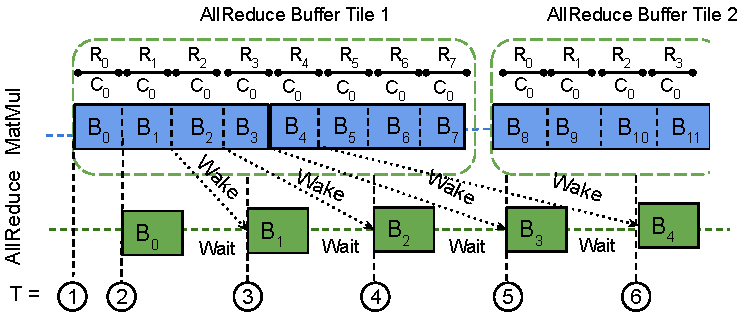
\includegraphics[width=\linewidth]{figures/overlap-example-rank-0.pdf}
    \caption{Workflow of overlap on \textbf{rank 0}. Rank 0 starts with chunk 0. }
	\end{subfigure}
    \hfill % \par \bigskip% Do not remove this. Without this there is no space between caption of above figure and the next figure. WEIRD bug. Never saw this in subfigure.
    \begin{subfigure}{0.48\linewidth}
    	\centering
        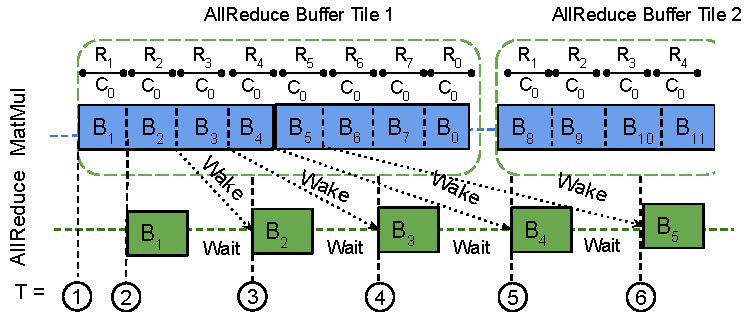
\includegraphics[width=\linewidth]{figures/overlap-example-rank-1.pdf}
        \caption{Workflow of overlap on \textbf{rank 1}. Rank 1 starts with chunk 1. }
    \end{subfigure}

	\caption{Workflow of \tool's overlapping of MatMul with \allreduce for a Float 16 matrix [8192, 3072] on 8 ranks (R$_0$ to R$_7$) with 1 channel (C$_0$) and 16 MB buffer size. Size of each 2-D chunk (B$_0$ to B$_{15}$) is [1024, 1024]. \tool's \allreduce and MatMul enables overlapping without decreasing the communication bandwidth and the efficiency of computation kernels.\label{fig:workflow-overlap}}
\end{figure*}

\subsection{Overlapping of Communication and Computation}
\label{sec:overlap-impl}
Overlapping of computation and communication has been studied in the context of executing stencil computations in a distributed system~\cite{Barigou2017,6799131,10.1145/2503210.2503289, 7573826,distributed-halide,KOZIRIS20031138,7336201,10.1145/1810085.1810091,8121995,10.1007/978-3-319-58667-0_18,sc20:pencil}.
These works use non-blocking MPI operations to communicate data and simultaneously perform computations on CPUs.
A similar approach for overlapping of computation and communication operations for a GPU workload would involve dividing all operations into sub-operations and ensuring dependency between sub-operations using CUDA streams.
However, this approach would provide sub-optimal performance because each sub-operation is performed on only a part of data, which leads to in-efficient computation and under-utilization of communication bandwidth.

%\tool's overlapping approach solves the issues of the traditional approach 
%We explain how \tool addresses this issue using example of GEMM and \allreduce.
Figure~\ref{fig:workflow-overlap} shows how the fine-grained overlapping of \tool addresses this issue using the example of a MatMul followed by a ring \allreduce.
First, it schedules the MatMul kernel (based on CUTLASS~\cite{cutlass})
to produce chunks in the same order as the \allreduce consumes them.
Here, the $n^{\text{th}}$ rank sends chunks in the order starting from the $n^{\text{th}}$ chunk. 
Hence, the MatMul kernel on $n^{\text{th}}$ rank produces chunks in the same order.
Second, \tool invokes both kernels only once on different streams and synchronizes the \allreduce with the MatMul using an efficient fine-grained spin-lock on a memory buffer to ensure that the \allreduce wakes up as soon as the MatMul produces a chunk.
% Since spin-lock requires all thread blocks to be running on a GPU, \tool{} generated \allreduce kernel uses grid strided loops to decrease the number of thread blocks to be invoked and invoke them using CUDA Grid Cooperative Groups.
Third, to provide opportunities to tune the 2-D tile sizes of the MatMul kernel, \tool generates a 2-D \allreduce kernel that communicates 2-D chunks, while NCCL \allreduce only supports 1-D continuous chunk.

%\allreduce kernel that communicates 2-dimensional chunks instead of 1-dimensional chunks in existing NCCL \allreduce kernel.

% \begin{figure*}[t]
% 	%https://docs.google.com/drawings/d/1yruTA_zsBAtsioXto2p7XsyDypk3WE8Dqx6Z4e9-35g/edit
% 	\begin{subfigure}{\linewidth}
% 		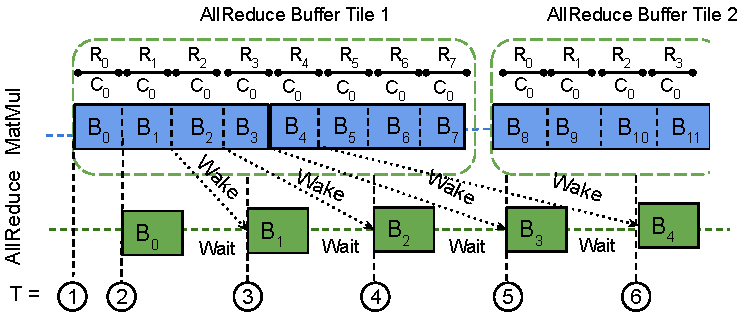
\includegraphics[width=\linewidth]{figures/overlap-example-rank-0.pdf}
% 		\caption{Workflow of overlap on \textbf{rank 0}. Rank 0 starts with chunks associated with Rank 0. }
% 	\end{subfigure}
	
% 	\begin{subfigure}{\linewidth}
% 		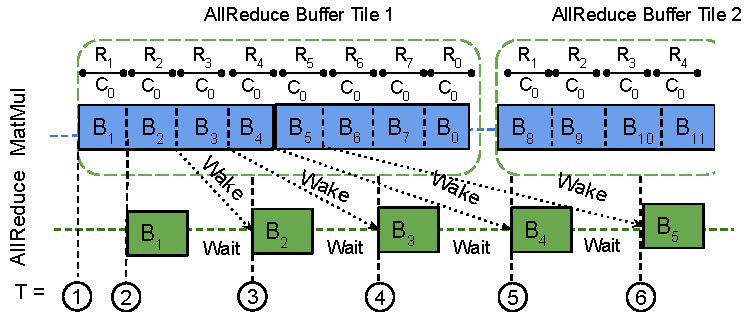
\includegraphics[width=\linewidth]{figures/overlap-example-rank-1.pdf}
% 		\caption{Workflow of overlap on \textbf{rank 1}. Rank 1 starts with chunks associated with Rank 1. }
% 	\end{subfigure}
% 	\caption{Workflow of \tool's overlapping of producer computation stage with a consumer \allreduce stage for data of size 128MB on 4 ranks (R$_0$ to R$_3$) with 2 channels (C$_0$ to C$_1$) and 64 MB buffer size. Size of each chunk is 8MB. \tool's custom communication kernel allows better overlapping without any decrease in communication bandwidth.
% 		\label{fig:workflow-overlap}}
% \end{figure*}

The example in Figure~\ref{fig:workflow-overlap} works as follows.
At T = \circled{1}, all ranks invoke MatMul and \allreduce kernels.
On rank 0, after computing chunk 0, the MatMul kernel wakes the \allreduce kernel at T = \circled{2}, which starts communicating chunk 0.
While on rank 1, at T = \circled{2} the MatMul kernel wakes the \allreduce kernel to communicate chunk 1.
%In parallel, the GEMM kernels on both ranks compute next chunks.
Concurrently, both MatMul kernels compute their corresponding next chunk.
At T = \circled{3}, MatMul kernels finished computing chunk 1 on rank 0 and chunk 2 on rank 1 and wakes up corresponding \allreduce kernels to communicate these chunks.
% Meanwhile, the GEMM kernel produces next chunks required by \allreduce.
This process continues until all chunks are processed.
%This process continues until the GEMM kernel finishes all chunks.

This process allows the MatMul kernel and \allreduce to be overlapped in a fine-grained manner,
which reduces the startup latency of \allreduce.
Since \allreduce communicates on the same chunk sizes, it achieves maximum communication bandwidth.
Furthermore, the MatMul kernel achieves maximum efficiency because the kernel is invoked on the full matrix size.
Figure~\ref{fig:matmul-overlap-intro} shows that this overlapping provides up to 1.36$\times$ better performance and hides more than 80\% of the MatMul time.

\subsection{Operations on Scattered Tensors}
\label{sec:scattered-tensors}
In data parallelism, communication and computation occur on different layers of widely different sizes.
Since machine learning frameworks allocate parameters and gradients of layers in non-contiguous buffers,
gradients are copied to a large buffer to avoid launching multiple \allreduce operations.
% The flatten and unflatten operations in Figure~\ref{fig:motivation} exemplify this problem.

\tool supports generating a single kernel for both computation and communication operations acting on non-contiguous tensors.
In this section, we show how \tool modifies NCCL to generate a single communication kernel for scattered tensors.
This code generation is non-trivial because NCCL has several design decisions based on the assumption that it is communicating a single contiguous buffer.
For example, each thread of a NCCL channel copies only a few elements in each iteration, and hence indexing the correct tensor at a particular offset requires a linear search through all non-contiguous tensors, which can lead to significant overhead.
\tool solves this problem by first dividing each tensor into buckets of size at most 2$^{10}$ elements and then assigning buckets to warps in a round-robin manner.
This mechanism allows each thread to quickly find the offset in a tensor, since a warp can directly index in its assigned bucket.
\tool pre-calculates the number of buckets that belong to the same contiguous buffer and calculates the offset for all of them once.

The process of breaking each tensor to buckets has computation overhead and extra memory requirements.
Since this bucketing is done only once on the CPU and training tasks run for thousands of iterations on the same tensors, the computation overhead is negligible.
Each bucket is represented by a pair of 64-bit tensor address and a 32-bit offset into the associated tensor, leading to $12 \times \left \lceil \frac{N}{2^{10}}\right \rceil$ bytes of extra memory for a tensor with $N$ elements.
However, this memory overhead is negligible for large models. For example, for BERT model with 334M elements, the memory requirement is 0.6\%.
Table~\ref{tab:scattered-tensors} shows that the overhead of scattered tensors is insignificant over contiguous tensors.

\begin{table}[t]
    \center
  \small
  \caption{Time to perform parameter update of all 360 tensors of BERT using Adam/LAMB on 256 Tesla V100 GPUs with scattered tensors implementation and a single contiguous tensor of size equal to the sum of size of all tensors.\label{tab:scattered-tensors}}
  \begin{tabular}{c|c|l}
  \textbf{Optimizer}   & \textbf{Scattered Tensor} & \textbf{Single Tensor}\\ \hline
  Adam & 33.89 ms & 33.21 ms  \\ 
  LAMB & 37.04 ms & 36.71 ms
  \end{tabular}
  \par \bigskip% Do not remove this. Without this there is no space between caption and the table
\end{table}

\subsection{PyTorch Integration}
\label{sec:pytorch-integration}
We integrated \tool generated code as a function to PyTorch's \texttt{torch.distributed} module.
This design allows us to re-use the logic for initializing NCCL and provide compatibility with models already using \texttt{torch.distributed}.
We added wrapper functions for calling \tool generated operations.
These wrapper functions prepare the arguments for calling \tool's operations, which includes pre-calculating pointers to the buckets for scattered tensors and clearing the spin-lock buffers for overlapping.
Machine learning models can invoke \tool functions using PyTorch.